
%% bare_conf.tex
%% V1.4
%% 2012/12/27
%% by Michael Shell
%% See:
%% http://www.michaelshell.org/
%% for current contact information.
%%
%% This is a skeleton file demonstrating the use of IEEEtran.cls
%% (requires IEEEtran.cls version 1.8 or later) with an IEEE conference paper.
%%
%% Support sites:
%% http://www.michaelshell.org/tex/ieeetran/
%% http://www.ctan.org/tex-archive/macros/latex/contrib/IEEEtran/
%% and
%% http://www.ieee.org/

%%*************************************************************************
%% Legal Notice:
%% This code is offered as-is without any warranty either expressed or
%% implied; without even the implied warranty of MERCHANTABILITY or
%% FITNESS FOR A PARTICULAR PURPOSE! 
%% User assumes all risk.
%% In no event shall IEEE or any contributor to this code be liable for
%% any damages or losses, including, but not limited to, incidental,
%% consequential, or any other damages, resulting from the use or misuse
%% of any information contained here.
%%
%% All comments are the opinions of their respective authors and are not
%% necessarily endorsed by the IEEE.
%%
%% This work is distributed under the LaTeX Project Public License (LPPL)
%% ( http://www.latex-project.org/ ) version 1.3, and may be freely used,
%% distributed and modified. A copy of the LPPL, version 1.3, is included
%% in the base LaTeX documentation of all distributions of LaTeX released
%% 2003/12/01 or later.
%% Retain all contribution notices and credits.
%% ** Modified files should be clearly indicated as such, including  **
%% ** renaming them and changing author support contact information. **
%%
%% File list of work: IEEEtran.cls, IEEEtran_HOWTO.pdf, bare_adv.tex,
%%                    bare_conf.tex, bare_jrnl.tex, bare_jrnl_compsoc.tex,
%%                    bare_jrnl_transmag.tex
%%*************************************************************************

% *** Authors should verify (and, if needed, correct) their LaTeX system  ***
% *** with the testflow diagnostic prior to trusting their LaTeX platform ***
% *** with production work. IEEE's font choices can trigger bugs that do  ***
% *** not appear when using other class files.                            ***
% The testflow support page is at:
% http://www.michaelshell.org/tex/testflow/



% Note that the a4paper option is mainly intended so that authors in
% countries using A4 can easily print to A4 and see how their papers will
% look in print - the typesetting of the document will not typically be
% affected with changes in paper size (but the bottom and side margins will).
% Use the testflow package mentioned above to verify correct handling of
% both paper sizes by the user's LaTeX system.
%
% Also note that the "draftcls" or "draftclsnofoot", not "draft", option
% should be used if it is desired that the figures are to be displayed in
% draft mode.
%
\documentclass[conference]{IEEEtran}
% Add the compsoc option for Computer Society conferences.
%
% If IEEEtran.cls has not been installed into the LaTeX system files,
% manually specify the path to it like:
% \documentclass[conference]{../sty/IEEEtran}





% Some very useful LaTeX packages include:
% (uncomment the ones you want to load)


% *** MISC UTILITY PACKAGES ***
%
%\usepackage{ifpdf}
% Heiko Oberdiek's ifpdf.sty is very useful if you need conditional
% compilation based on whether the output is pdf or dvi.
% usage:
% \ifpdf
%   % pdf code
% \else
%   % dvi code
% \fi
% The latest version of ifpdf.sty can be obtained from:
% http://www.ctan.org/tex-archive/macros/latex/contrib/oberdiek/
% Also, note that IEEEtran.cls V1.7 and later provides a builtin
% \ifCLASSINFOpdf conditional that works the same way.
% When switching from latex to pdflatex and vice-versa, the compiler may
% have to be run twice to clear warning/error messages.






% *** CITATION PACKAGES ***
%
%\usepackage{cite}
% cite.sty was written by Donald Arseneau
% V1.6 and later of IEEEtran pre-defines the format of the cite.sty package
% \cite{} output to follow that of IEEE. Loading the cite package will
% result in citation numbers being automatically sorted and properly
% "compressed/ranged". e.g., [1], [9], [2], [7], [5], [6] without using
% cite.sty will become [1], [2], [5]--[7], [9] using cite.sty. cite.sty's
% \cite will automatically add leading space, if needed. Use cite.sty's
% noadjust option (cite.sty V3.8 and later) if you want to turn this off
% such as if a citation ever needs to be enclosed in parenthesis.
% cite.sty is already installed on most LaTeX systems. Be sure and use
% version 4.0 (2003-05-27) and later if using hyperref.sty. cite.sty does
% not currently provide for hyperlinked citations.
% The latest version can be obtained at:
% http://www.ctan.org/tex-archive/macros/latex/contrib/cite/
% The documentation is contained in the cite.sty file itself.






% *** GRAPHICS RELATED PACKAGES ***
%
\ifCLASSINFOpdf
  % \usepackage[pdftex]{graphicx}
  % declare the path(s) where your graphic files are
  % \graphicspath{{../pdf/}{../jpeg/}}
  % and their extensions so you won't have to specify these with
  % every instance of \includegraphics
  % \DeclareGraphicsExtensions{.pdf,.jpeg,.png}
\else
  % or other class option (dvipsone, dvipdf, if not using dvips). graphicx
  % will default to the driver specified in the system graphics.cfg if no
  % driver is specified.
  % \usepackage[dvips]{graphicx}
  % declare the path(s) where your graphic files are
  % \graphicspath{{../eps/}}
  % and their extensions so you won't have to specify these with
  % every instance of \includegraphics
  % \DeclareGraphicsExtensions{.eps}
\fi
% graphicx was written by David Carlisle and Sebastian Rahtz. It is
% required if you want graphics, photos, etc. graphicx.sty is already
% installed on most LaTeX systems. The latest version and documentation
% can be obtained at: 
% http://www.ctan.org/tex-archive/macros/latex/required/graphics/
% Another good source of documentation is "Using Imported Graphics in
% LaTeX2e" by Keith Reckdahl which can be found at:
% http://www.ctan.org/tex-archive/info/epslatex/
%
% latex, and pdflatex in dvi mode, support graphics in encapsulated
% postscript (.eps) format. pdflatex in pdf mode supports graphics
% in .pdf, .jpeg, .png and .mps (metapost) formats. Users should ensure
% that all non-photo figures use a vector format (.eps, .pdf, .mps) and
% not a bitmapped formats (.jpeg, .png). IEEE frowns on bitmapped formats
% which can result in "jaggedy"/blurry rendering of lines and letters as
% well as large increases in file sizes.
%
% You can find documentation about the pdfTeX application at:
% http://www.tug.org/applications/pdftex





% *** MATH PACKAGES ***
%
%\usepackage[cmex10]{amsmath}
% A popular package from the American Mathematical Society that provides
% many useful and powerful commands for dealing with mathematics. If using
% it, be sure to load this package with the cmex10 option to ensure that
% only type 1 fonts will utilized at all point sizes. Without this option,
% it is possible that some math symbols, particularly those within
% footnotes, will be rendered in bitmap form which will result in a
% document that can not be IEEE Xplore compliant!
%
% Also, note that the amsmath package sets \interdisplaylinepenalty to 10000
% thus preventing page breaks from occurring within multiline equations. Use:
%\interdisplaylinepenalty=2500
% after loading amsmath to restore such page breaks as IEEEtran.cls normally
% does. amsmath.sty is already installed on most LaTeX systems. The latest
% version and documentation can be obtained at:
% http://www.ctan.org/tex-archive/macros/latex/required/amslatex/math/





% *** SPECIALIZED LIST PACKAGES ***
%
%\usepackage{algorithmic}
% algorithmic.sty was written by Peter Williams and Rogerio Brito.
% This package provides an algorithmic environment fo describing algorithms.
% You can use the algorithmic environment in-text or within a figure
% environment to provide for a floating algorithm. Do NOT use the algorithm
% floating environment provided by algorithm.sty (by the same authors) or
% algorithm2e.sty (by Christophe Fiorio) as IEEE does not use dedicated
% algorithm float types and packages that provide these will not provide
% correct IEEE style captions. The latest version and documentation of
% algorithmic.sty can be obtained at:
% http://www.ctan.org/tex-archive/macros/latex/contrib/algorithms/
% There is also a support site at:
% http://algorithms.berlios.de/index.html
% Also of interest may be the (relatively newer and more customizable)
% algorithmicx.sty package by Szasz Janos:
% http://www.ctan.org/tex-archive/macros/latex/contrib/algorithmicx/




% *** ALIGNMENT PACKAGES ***
%
%\usepackage{array}
% Frank Mittelbach's and David Carlisle's array.sty patches and improves
% the standard LaTeX2e array and tabular environments to provide better
% appearance and additional user controls. As the default LaTeX2e table
% generation code is lacking to the point of almost being broken with
% respect to the quality of the end results, all users are strongly
% advised to use an enhanced (at the very least that provided by array.sty)
% set of table tools. array.sty is already installed on most systems. The
% latest version and documentation can be obtained at:
% http://www.ctan.org/tex-archive/macros/latex/required/tools/


% IEEEtran contains the IEEEeqnarray family of commands that can be used to
% generate multiline equations as well as matrices, tables, etc., of high
% quality.




% *** SUBFIGURE PACKAGES ***
%\ifCLASSOPTIONcompsoc
%  \usepackage[caption=false,font=normalsize,labelfont=sf,textfont=sf]{subfig}
%\else
%  \usepackage[caption=false,font=footnotesize]{subfig}
%\fi
% subfig.sty, written by Steven Douglas Cochran, is the modern replacement
% for subfigure.sty, the latter of which is no longer maintained and is
% incompatible with some LaTeX packages including fixltx2e. However,
% subfig.sty requires and automatically loads Axel Sommerfeldt's caption.sty
% which will override IEEEtran.cls' handling of captions and this will result
% in non-IEEE style figure/table captions. To prevent this problem, be sure
% and invoke subfig.sty's "caption=false" package option (available since
% subfig.sty version 1.3, 2005/06/28) as this is will preserve IEEEtran.cls
% handling of captions.
% Note that the Computer Society format requires a larger sans serif font
% than the serif footnote size font used in traditional IEEE formatting
% and thus the need to invoke different subfig.sty package options depending
% on whether compsoc mode has been enabled.
%
% The latest version and documentation of subfig.sty can be obtained at:
% http://www.ctan.org/tex-archive/macros/latex/contrib/subfig/




% *** FLOAT PACKAGES ***
%
%\usepackage{fixltx2e}
% fixltx2e, the successor to the earlier fix2col.sty, was written by
% Frank Mittelbach and David Carlisle. This package corrects a few problems
% in the LaTeX2e kernel, the most notable of which is that in current
% LaTeX2e releases, the ordering of single and double column floats is not
% guaranteed to be preserved. Thus, an unpatched LaTeX2e can allow a
% single column figure to be placed prior to an earlier double column
% figure. The latest version and documentation can be found at:
% http://www.ctan.org/tex-archive/macros/latex/base/


%\usepackage{stfloats}
% stfloats.sty was written by Sigitas Tolusis. This package gives LaTeX2e
% the ability to do double column floats at the bottom of the page as well
% as the top. (e.g., "\begin{figure*}[!b]" is not normally possible in
% LaTeX2e). It also provides a command:
%\fnbelowfloat
% to enable the placement of footnotes below bottom floats (the standard
% LaTeX2e kernel puts them above bottom floats). This is an invasive package
% which rewrites many portions of the LaTeX2e float routines. It may not work
% with other packages that modify the LaTeX2e float routines. The latest
% version and documentation can be obtained at:
% http://www.ctan.org/tex-archive/macros/latex/contrib/sttools/
% Do not use the stfloats baselinefloat ability as IEEE does not allow
% \baselineskip to stretch. Authors submitting work to the IEEE should note
% that IEEE rarely uses double column equations and that authors should try
% to avoid such use. Do not be tempted to use the cuted.sty or midfloat.sty
% packages (also by Sigitas Tolusis) as IEEE does not format its papers in
% such ways.
% Do not attempt to use stfloats with fixltx2e as they are incompatible.
% Instead, use Morten Hogholm'a dblfloatfix which combines the features
% of both fixltx2e and stfloats:
%
% \usepackage{dblfloatfix}
% The latest version can be found at:
% http://www.ctan.org/tex-archive/macros/latex/contrib/dblfloatfix/




% *** PDF, URL AND HYPERLINK PACKAGES ***
%
%\usepackage{url}
% url.sty was written by Donald Arseneau. It provides better support for
% handling and breaking URLs. url.sty is already installed on most LaTeX
% systems. The latest version and documentation can be obtained at:
% http://www.ctan.org/tex-archive/macros/latex/contrib/url/
% Basically, \url{my_url_here}.

%*** para suportar acentuação ***
\usepackage[utf8]{inputenc}

%*** para suportar tabelas com colunas mergeadas ***
\usepackage{multirow}

%*** Para inclusão de imagens e permitir rotacionar texto ***
\usepackage{graphicx}			% Inclusão de gráficos
\graphicspath{ {./} }			% localizando as imagens

%*** Para ajustar a largura das colunas e para multilinhas nas células ***
\usepackage{array}
\newcolumntype{L}{>{\centering\arraybackslash}m{0,75cm}}
\newcolumntype{M}{>{\RaggedLeft\arraybackslash}m{3cm}}

% *** Do not adjust lengths that control margins, column widths, etc. ***
% *** Do not use packages that alter fonts (such as pslatex).         ***
% There should be no need to do such things with IEEEtran.cls V1.6 and later.
% (Unless specifically asked to do so by the journal or conference you plan
% to submit to, of course. )

\usepackage{xcolor}
\newcommand{\marcos}[1]{{\color{blue}{MARCOS: #1}}}
\newcommand{\marcosT}[1]{{\color{red}{TODO: #1}}}
\newcommand{\marcosR}[1]{{\color{brown}{COMMENT: #1}}}
\newcommand{\fancyname}{Dizang}
\newcommand{\fancynameX}{\fancyname}

%shortcuts
\newcommand{\xfig}{
\includegraphics[scale=0.007]{x.png}}
\newcommand{\checkfig}{
\includegraphics[scale=0.015]{check.png}}

% correct bad hyphenation here
\hyphenation{op-tical net-works semi-conduc-tor}


\begin{document}
%
% paper title
% can use linebreaks \\ within to get better formatting as desired
% Do not put math or special symbols in the title.
%\title{Coletando dados de memória de máquina em nuvem para análise forense de ataques de injeção de código}
\title{\fancynameX: Uma solução para coleta de evidências forenses de ataques de injeção na nuvem}


% author names and affiliations
% use a multiple column layout for up to three different
% affiliations
\author{\IEEEauthorblockN{Hamilton Fonte II, Marcos A. Simplicio Jr.}
\IEEEauthorblockA{
Escola Politécnica, Universidade de São Paulo (USP)
São Paulo, SP, Brasil\\
Email: hamiltonii@gmail.com, mjunior@larc.usp.br}
%\and
%\IEEEauthorblockN{Marcos A. Simplicio Jr.}
%\IEEEauthorblockA{
%Escola Politécnica -- Universidade de São Paulo (USP)
%São Paulo, SP, Brasil\\
%Email: mjunior@larc.usp.br}
}

% conference papers do not typically use \thanks and this command
% is locked out in conference mode. If really needed, such as for
% the acknowledgment of grants, issue a \IEEEoverridecommandlockouts
% after \documentclass

% for over three affiliations, or if they all won't fit within the width
% of the page, use this alternative format:
% 
%\author{\IEEEauthorblockN{Michael Shell\IEEEauthorrefmark{1},
%Homer Simpson\IEEEauthorrefmark{2},
%James Kirk\IEEEauthorrefmark{3}, 
%Montgomery Scott\IEEEauthorrefmark{3} and
%Eldon Tyrell\IEEEauthorrefmark{4}}
%\IEEEauthorblockA{\IEEEauthorrefmark{1}School of Electrical and Computer Engineering\\
%Georgia Institute of Technology,
%Atlanta, Georgia 30332--0250\\ Email: see http://www.michaelshell.org/contact.html}
%\IEEEauthorblockA{\IEEEauthorrefmark{2}Twentieth Century Fox, Springfield, USA\\
%Email: homer@thesimpsons.com}
%\IEEEauthorblockA{\IEEEauthorrefmark{3}Starfleet Academy, San Francisco, California 96678-2391\\
%Telephone: (800) 555--1212, Fax: (888) 555--1212}
%\IEEEauthorblockA{\IEEEauthorrefmark{4}Tyrell Inc., 123 Replicant Street, Los Angeles, California 90210--4321}}




% use for special paper notices
%\IEEEspecialpapernotice{(Invited Paper)}




% make the title area
\maketitle

% As a general rule, do not put math, special symbols or citations
% in the abstract
\begin{abstract}
A adoção de arquiteturas em nuvem aumenta a cada dia, e com ela também o número de casos em que esse tipo de tecnologia é usada para fins ilícitos. 
%
Infelizmente, devido à natureza volátil da nuvem, a tarefa de coletar evidências para análise forense nesse ambiente tem esbarrado em desafios práticos e legais.
%
Este trabalho analisa propostas na literatura voltadas a resolver os principais desafios existentes na coleta evidências na nuvem, discutindo suas limitações, e então propõe uma solução que cobre coleta, transporte e armazenamento da evidência visando suplantá-las. 
%
A solução aqui proposta provê uma forma de correlacionar evidências e sua origem virtual, permitindo transportar e armazenar tais dados sem afetar sua credibilidade.
%
Especificamente, ela tem como focos (1) a reprodutibilidade do processo de coleta e (2) a garantia de custódia da evidência.

\end{abstract}

% no keywords




% For peer review papers, you can put extra information on the cover
% page as needed:
% \ifCLASSOPTIONpeerreview
% \begin{center} \bfseries EDICS Category: 3-BBND \end{center}
% \fi
%
% For peerreview papers, this IEEEtran command inserts a page break and
% creates the second title. It will be ignored for other modes.
\IEEEpeerreviewmaketitle

\section{Introdução}

%==== CONTEXTO GERAL: Nuvem e volatilidade de VMs ====
%
Técnicas de virtualização, replicação de serviços e compartilhamento de recursos entre múltiplos usuários (multi-inquilinato) proveem a nuvens computacionais uma elevada escalabilidade \cite{Morsy_Cloud_Security:2010}.
%
Ao mesmo tempo, tais mecanismos também criam uma elevada volatilidade dos recursos virtuais que executam aplicações em nuvem.
%
Afinal, quando submetida a uma carga elevada, uma aplicação hospedada na nuvem pode criar clones das máquinas virtuais (\textit{virtual machines} -- VMs) que a hospedam e balancear a carga entre elas, de modo a atender à demanda sem prejuízos na qualidade do serviço oferecido. 
%
Após esse pico, as máquinas que foram clonadas são normalmente desativadas, seus recursos liberados e o sistema retorna à capacidade anterior, evitando-se custos desnecessários


%==== CONTEXTO ESPECÍFICO + PROBLEMA GERAL: Forense na nuvem vs. volatilidade + multitenancy + multidomains ====
%
Embora interessante do ponto de vista de eficiência e custos, do ponto de vista forense a volatilidade da nuvem traz problemas em caso de ataques.
%
Por exemplo, caso uma das instâncias de processamento virtuais criadas temporariamente seja alvo de ameaças que atuam diretamente na sua memória, sem deixar rastros em discos (e.g., arquivos de \textit{log}), as evidências desse evento podem ser completamente perdidas após elas serem desativadas e terem seus recursos liberados.
%
Essa dificuldade é ainda agravada por aspectos como multi-inquilinato e multi-jurisdição típicas de soluções em nuvem \cite{Bash_Adv_in_Forensics:2015}.
%
Especificamente, o aspecto multi-inquilino dificulta a obtenção do \textit{hardware} que executa as aplicações de interesse, pois, como ele é compartilhado por vários usuários, removê-los para análise poderia levar a uma violação de privacidade dos usuários não relacionados à investigação. 
%
Já a natureza distribuída da nuvem pode levar à alocação de informações relevantes à investigação em vários países, dificultando a obtenção das mesmas em especial quando não existem acordos de cooperação entre as entidades envolvidas \cite{Dykstra_Acquiring_for_IAAS:2012}.
%
Combinadas, tais características dificultam a coleta de evidências com a credibilidade necessária para que elas possam ser usadas em processos legais,  o que exige o respeito à privacidade, à jurisdição e à cadeia de custódia, bem como a reprodutibilidade do processo de coleta \cite{Rahman_Live_Forensics_Techniques:2015}.


%==== O QUE EXISTE E PORQUE NÃO É SUFICIENTE: ??? ====
%
Embora existam soluções na literatura que abordam a coleta de informações de nuvem com o propósito de análise forense, a grande maioria delas aborda a coleta, o transporte e o armazenamento de forma isolada.
%
Por exemplo, trabalhos como \cite{Dykstra_FROST:2013} e \cite{Reichert_Auto_acquisition:2015} tratam de fatores como multi-inquilinato e multi-jurisdição, discutindo formas de coleta e preservação da evidência fora da nuvem.
%
Já estudos como \cite{George_DF2CE:2012} se concentram na análise forense para a coleta de evidência de máquinas virtuais enquanto elas estão em execução, enquanto trabalhos como \cite{Sang_Log_approach:2013} abordam a questão de processos de garantia de cadeia de custódia em ambientes de nuvem para transporte da evidência.
%
%abordam os problemas descritos anteriormente \marcosT{QUAIS, CARA PÁLIDA? VOCÊ LISTOU 4 TIPOS DE ATAQUE E DEIXOU UM PROBLEMA GERAL: COMO O LEITOR VAI SABER QUAIS EXATAMENTE SÃO ABORDADOS? Seja mais preciso: clareza acima de tudo!!!} de forma isolada.
%
%Alguns propõem soluções para o os fatores multi-inquilino e multi-jurisdição, outros abordam apenas a coleta de evidência de máquinas virtuais e por fim temos as que descrevem apenas os processos de garantia de cadeia de custodia. \marcosT{Er... você não me deu sequer um exemplo, então eu sou obrigado a acreditar em você sem que você apresente argumentos... lembre-se que revisores são seres amargos e cruéis, que não acreditam em nada, então melhor não arriscar e dar exemplos claros.}
%
Por outro lado, não foram identificadas na literatura propostas que (1) descrevam como o dado é coletado e armazenado observando a cadeia de custódia, e (2) visem garantir que, mesmo que um recurso virtualizado (e.g., uma VM) seja desalocada, haja condições de se reproduzir o processo de coleta de evidências.



%==== O QUE FAZEMOS: Ataques de injeção ====
%
O presente trabalho visa suplantar tais limitações por meio de uma proposta que tem como focos (1) a reprodutibilidade do processo de coleta, (2) o estabelecimento de vínculo entre a evidência coletada e sua origem, (3) a preservação da jurisdição e da privacidade dos não envolvidos na investigação e (4) a garantia de custódia da evidência.
%
Em suma, a solução descrita provê uma forma de correlacionar evidências e sua origem virtual, permitindo transportar e armazenar tais dados de modo a preservar sua credibilidade.
%
Para isso, a proposta supõe que o sistema sendo monitorado é executado dentro de um contêiner em nuvem. 
%
O foco da solução em contêiner se justifica pelo crescimento da adoção de conteinerização nos últimos anos, bem como pela previsão de que este será o modelo de implementação mais usado em aplicações futuras \cite{Piraghaj_Container_Cloud_Computing:2016}.
%
A solução tem como alvo específico ataques de injeção de código \cite{Case_Memory_Forensics:2014}, pois estes, quando usados contra uma arquitetura em nuvem, não deixam rastros quando recursos de processamento virtuais são desativados e sua memória é liberada \cite{Vomel_Memory_Acquisition:2013}, \cite{Case_Memory_Forensics:2014}.
%
Em particular, têm especial interesse quatro tipos específicos dessa família de ameaças \cite{Case_Memory_Forensics:2014}:


\begin{itemize}
 \item \textbf{Injeção remota de bibliotecas}: Um processo malicioso força o processo alvo a carregar uma biblioteca em seu espaço de memória.
 %
 Como resultado, o código da biblioteca carregada executa com os mesmos privilégios do executável em que ela foi injetada. 
 %
 Esta estratégia, comumente usada para instalar malwares, pode fazer com que uma biblioteca maliciosa armazenada no sistema seja distribuída por vários processos de uma mesma máquina, dificultando sua remoção \cite{Miller_Remote_Library_Injection:2004}.
 %
 \item \textbf{Inline Hooking}: Um processo malicioso escreve código como uma sequência de bytes diretamente no espaço de memória de um processo alvo, e então força este último a executar o código injetado. 
 %
 O código pode ser, por exemplo, um \textit{script} de \textit{shell}.
 %
 \item \textbf{Injeção reflexiva de biblioteca}: Um processo malicioso acessa diretamente a memória do processo alvo, inserindo nela o código de uma biblioteca na forma de uma sequência de bytes, e então força o processo a executar essa biblioteca. 
 %
 Nessa forma de ataque, a biblioteca maliciosa não existe fisicamente; isso torna tal estratégia de injeção de código potencialmente mais atrativa, pois o carregamento da biblioteca não é registrado no sistema operacional (SO), dificultando a detecção do ataque \cite{Fewer_Reflective_Library_Inject:2008}.
 %
 \item \textbf{Injeção de processo vazio}: Um processo malicioso dispara uma instância de um processo legítimo no estado ``suspenso''; a área do executável é então liberada e realocada com código malicioso.
\end{itemize}


O restante deste documento está organizado da seguinte forma.
%
A Seção \ref{sec:cloud} discute brevemente soluções em nuvem e suas características.
%
A Seção \ref{sec:related} analisa os trabalhos relacionados na área de forense de memória.
%
A Seção \ref{sec:proposal} detalha a solução proposta e avalia como ela trata os desafios alvo deste projeto.
%
Finalmente, a Seção \ref{sec:conclusion} apresenta algumas considerações finais e discute ideias para trabalhos futuros.


\section{Adoção de arquiteturas em nuvem e contêineres}
\label{sec:cloud}


Uma nuvem computacional é um modelo de infraestrutura no qual recursos compartilhados em quantidade configurável, acessíveis via rede, são alocados e desalocados com esforço mínimo de gerenciamento por parte de um provedor de serviços. \cite{NIST2011}
%A infraestrutura é composta de máquinas físicas contendo cada uma um número variável de máquinas virtuais que implementam este serviço \cite{Sousa_Computacao_Nuvem:2009}. 
%
Há três modelos principais de comercialização de uso da nuvem \cite{NIST2011}: \textit{software} como serviço (\textit{Software as a Service} -- SaaS), na qual se provê o \textit{software} que será usado pelo cliente; plataforma como serviço (\textit{Platform as a Service} -- PaaS), na qual se provê o ambiente para que o cliente desenvolva, teste e execute seu \textit{software}; e, o tipo mais pertinente para este trabalho, Infraestrutura como serviço (\textit{Infrastructure as a Service} -- IaaS), na qual são fornecidos recursos computacionais básicos, como processamento e memória, em geral de forma virtualizada.


A virtualização de recursos na nuvem, embora tradicionalmente feita por meio de máquinas virtuais, vêm sendo crescentemente feita também na forma de contêineres.
%
De fato, segundo o ``Container Market Adoption Survey 2016'', realizado pelas empresas DevOps.com (https://devops.com/) e ClusterHQ (https://clusterhq.com) com 235 empresas que têm desenvolvimento de software como sua atividade fim ou como suporte à atividade fim, 76\% dos respondentes utilizam contêiners para melhorar a eficiência do processo de desenvolvimento e em suas arquiteturas de micro-serviços em nuvem.
%
Diferentemente de máquinas virtuais, que envolvem a criação de um \textit{hardware} virtual e de um sistema operacional (SO) acima do sistema nativo e que opera independente deste, a virtualização com contêineres é feita no nível do SO nativo, tem uma implementação mais simples eliminado camadas entre o aplicativo executado e o \textit{hardware} físico.
%
Uma tecnologia bastante utilizada para esse propósito são Contêiners Linux (LXC) \cite{Linuxcontainers.org2015}, que aproveitam-se de funcionalidades como cgroups e namespacing do kernel do Linux para auxiliar no gerenciamento e isolamento de recursos virtuais.



\section{Trabalhos relacionados}
\label{sec:related}

Existem vários aspectos relativos à análise forense na nuvem, indo desde a coleta de informações até a garantia da cadeia de custódia de evidências.
%
Para uma discussão mais estruturada dos trabalhos disponíveis na literatura sobre o tema, a seguir eles são apresentados com base nos diferentes aspectos que abordam.

\subsection{Acessar e coletar as informações de memória das máquinas virtuais em nuvem}

Diversos trabalhos de análise forense na nuvem se concentram na coleta de dados ``após o fato'', ou seja, após a intrusão ser detectada \cite{Reichert_Auto_acquisition:2015,Poisel_VMI:2013,Dykstra_FROST:2013,George_DF2CE:2012,Sang_Log_approach:2013}. 
%
Os processos de coleta descritos nesses trabalhos podem ser iniciados de forma manual ou automaticamente, via integração com um mecanismo de detecção de intrusão. 
%
No caso específico de memória volátil, tal forma de coleta não consegue descrever como era a memória antes da intrusão, pois o processo só é acionado depois da detecção do ataque. 
%
%A capacidade de saber como era a memória antes do fato é descrita por \cite{Case_Memory_Forensics:2014} como necessária para viabilizar a abordagem de coletar o suficiente para realizar a investigação pois permite comparar dois instantâneos de memória e minimizar o volume coletado antes do fato. 
Tal limitação pode trazer prejuízos à investigação, dado que algumas análises dependem exatamente da capacidade de se comparar dois momentos da memória \cite{Case_Memory_Forensics:2014}. 
%
Entre os trabalhos estudados, a única proposta encontrada que leva tal necessidade em consideração é \cite{Dezfouli_Backup_approach:2012}, que propõe que o dado seja armazenado no próprio equipamento sob análise.
%
%Infelizmente, entretanto, essa abordagem não é aplicável ao cenário em nuvem, pois leva a perda de informações importantes caso a máquina virtual seja despejada e seus recursos liberados.
Infelizmente, entretanto, a aplicação de tal abordagem no cenário em nuvem é pouco viável, pois pode levar à perda de informações importantes caso a máquina virtual ou contêiner seja desativada, tendo seus recursos liberados.
%

%Ainda na coleta de informações, os autores \cite{Reichert_Auto_acquisition:2015} e \cite{George_DF2CE:2012} sugerem a abordagem de forense ao vivo onde os dados são constantemente coletados sem distinção do antes ou depois do fato. 
Existem ainda trabalhos voltados à coleta de informações durante a execução do sistema, nos quais os dados são constantemente coletados sem distinção do que aconteceu antes ou depois do fato de interesse.
%
Esse é o caso de trabalhos como \cite{Poisel_VMI:2013,Dykstra_FROST:2013,Sang_Log_approach:2013}, que adotam a estratégia de isolar e parar a máquina virtual para em seguida realizar o processo de coleta. 
%
%Nas duas estratégias citadas anteriormente, o problema do grande volume de informações coletadas não é abordado pelo autores nem o cenário onde é necessário coletar evidências de uma máquina virtual que já foi despejada do pool e os recursos liberados. 
Embora interessantes, as abordagens descritas nesses trabalhos podem levar a um elevado volume de dados coletados, além de também não tratarem o cenário em que é necessário coletar evidências quando os recursos virtuais contendo tais informações são liberados.


\subsection{Capacidade de reproduzir o processo e obter os mesmos resultados}

Se, durante uma análise forense, analistas diferentes obtêm resultados distintos ao executar o mesmo procedimento de coleta, a evidência gerada não tem credibilidade, inviabilizando seu uso em um processo legal. 
%
Por essa razão, a reprodutibilidade do processo de coleta é uma parte importante da geração de evidências para análise forense.
%
Infelizmente, entretanto, nenhuma das propostas encontradas na literatura atualmente permite tal reprodutibilidade em cenários de nuvem em que máquinas virtuais ou contêineres são desativados e seus recursos físicos liberados: todas elas dependem da existência do recurso virtual para a repetição do processo de coleta.

\subsection{Não violar privacidade ou jurisdição das partes não envolvidas na investigação}

Em um ambiente de nuvem pública, remover o \textit{hardware} para análise posterior pode levar à violação de privacidade de usuários, uma vez que o multi-inquilinato desse cenário faz com que uma mesma máquina física guarde informações de diversos clientes, alguns dos quais podem não estar envolvidos na investigação em curso.
%
Diversos trabalhos na literatura tratam esse problema adequadamente, por meio das duas estratégias principais: a primeira, adotada em \cite{Reichert_Auto_acquisition:2015,George_DF2CE:2012,Poisel_VMI:2013,Dykstra_FROST:2013}, consiste em coletar dados pertinentes à investigação e armazená-los fora da nuvem; a segunda, empregada em \cite{Sang_Log_approach:2013} e que constitui um caso específico de \cite{George_DF2CE:2012}, depende da cooperação do provedor de serviços de nuvem para conseguir as informações necessárias à investigação. 
%
Depender do provedor de serviços de nuvem é uma estratégia pouco recomendada, entretanto, pois (1) o volume de dados de usuários pode forçar os provedores a limitar o tamanho dos \textit{logs} armazenados, e (2) caso ocorra uma indisponibilidade causada por um ataque, o objetivo do provedor será o de restabelecer o serviço, não necessariamente o de preservar evidências\cite{Clarke_Review_of_Challenges:2015}. 


\subsection{Garantir a cadeia de custódia da evidência}

Dentre os trabalhos analisados, apenas \cite{Sang_Log_approach:2013} aborda a questão da garantia da cadeia de custódia. 
%
Especificamente, o trabalho emprega \textit{hashes} para verificar a integridade da evidência, permitindo a detecção de alterações na mesma, embora não explique os mecanismos que poderiam ser utilizados para impedir acesso não autorizado (e, assim, potencial alteração) aos próprios hashes. 
%
As propostas dos outros autores concentram-se apenas no aspecto técnico da coleta, sem discutir claramente garantia de custódia mas apenas mencionando que as evidências devem ser coletadas de forma ``forensicamente aceitável''.

\subsection{Resumo}

A Tabela \ref{tab:related-work} mostra um comparativo das soluções estudadas, considerando os aspectos discutidos nesta seção, posicionando as contribuições da proposta apresentada neste trabalho.

\begin{table}[htb!]
\centering
\caption{Comparativo de soluções de coleta de informações de memória de máquinas em nuvem para análise forense}
\label{tab:related-work}
\renewcommand{\arraystretch}{2}
\begin{tabular}{p{3.0cm}|L|L|L|L}
\cline{2-5}
\textbf{}															& \rotatebox{90}{\textbf{Coleta  é contínua?}}      & \rotatebox{90}{\textbf{Reproduz o processo sem a VM?}} & \rotatebox{90}{\textbf{Garante cadeia de custódia?}}     		& \rotatebox{90}{\textbf{Preserva jurisdição e privacidade?}}          \\ \hline
\fancyname (esta proposta)						& \checkfig	  & \checkfig               & \checkfig                  & \checkfig                             \\ \hline
\cite{George_DF2CE:2012}							& \xfig		  	& \xfig                   & \xfig                      & \checkfig                             \\ \hline
\cite{Poisel_VMI:2013}								& \xfig       & \xfig                   & \xfig                      & \checkfig                             \\ \hline
\cite{Dykstra_FROST:2013}							& \xfig       & \xfig                   & \xfig                      & \checkfig                             \\ \hline
\cite{Do_Desafio:2014}								& \xfig		    & \xfig                   & \xfig                      & \checkfig                             \\ \hline
\cite{Reichert_Auto_acquisition:2015}	& \xfig  	    & \xfig                   & \checkfig                  & \checkfig                             \\ \hline
\cite{Sang_Log_approach:2013}					& \checkfig   & \xfig	             			& \checkfig                  & \checkfig                             \\ \hline
\cite{Dolan-Gavitt_Semantic_Gap:2011}	& \xfig       & \xfig                   & \xfig                      & \checkfig                             \\ \hline
\cite{Aljaedi_Comparative:2011}				& \xfig       & \xfig                   & \xfig                      & \checkfig                             \\ \hline
\cite{Dezfouli_Backup_approach:2012}	& \checkfig   & \xfig                   & \xfig                      & \checkfig                             \\ \hline
\cite{VanBaar_FAAS:2014}							& \checkfig   & \xfig                   & \checkfig                  & \checkfig                             \\
\end{tabular}
\end{table}

\section{Solução proposta: \fancyname}
\label{sec:proposal}

A presente proposta tem como objetivo principal coletar memória de recursos computacionais virtuais de modo a conseguir: 
(1) identificar a fonte da evidência, mesmo se o recurso virtual não existir mais; 
(2) descrever o sistema antes e depois do incidente;
(3) transportar e armazenar a memória coletada de uma forma que garanta sua integridade e confidencialidade; e
(4) não violar a jurisdição e a privacidade de outros usuários que porventura tenham recursos alocados no mesmo servidor físico.
%
A solução aqui apresentada, denominada \fancyname, é descrita em detalhes a seguir.


\subsection{Descrição}

Em sistemas computacionais executados sobre uma infraestrutura física (i.e., não virtualizada), pode-se fazer uma associação direta entre um recurso qualquer, como uma informação da memória, imagem de disco ou pacotes trafegando na rede, e sua origem correspondente.
%
Já em sistemas construídos sobre uma infraestrutura virtual, em especial quando esta é auto-escalável, os recursos computacionais são altamente voláteis e, portanto, podem ser desalocados a qualquer momento.
%
Para conseguir correlacionar uma evidência a sua origem volátil, é necessário utilizar outro elemento em que persista a relação fonte-evidência, o que na presente proposta é feito por meio de contêineres linux (LXC).
%
Embora um contêiner seja um \textit{software} e, portanto, também volátil, cada imagem compilada e sua execução na forma de contêiner são normalmente atrelados a um \textit{hash} que identifica univocamente essa relação.
%
O contêiner também permite identificar com mais precisão a fonte de uma evidência, uma vez que é possível dividir as partes de um sistema em contêineres: por exemplo, um contêiner para o motor de páginas dinâmicas (e.g., Apache \cite{Tomcat}), outro com a lógica de negócios (e.g., \textit{golang} \cite{Google}) e um terceiro para um banco de dados (e.g., \textit{Cassandra} \cite{Cassandra}).

%\marcosT{O parágrafo estava muito grande, então quebrei aqui. O problema é que falta uma frase para ligar a frase a seguir ao contexto da discussão... Coloque uma frase aqui, deixando claro qual requisito você quer satisfazer com essa ideia de ``interromper temporariamente a execução do contêiner''. Aplique isso para TUDO que for proposta: o leitor tem que saber de antemão pra que você está fazendo alguma coisa, ou vai ficar se perguntando ``Espera, mas pra que fazer isso?!'' - Hamilton: Feito}
A cópia de memória não é uma atividade atômica, pois ela é executada em conjunto com outros processos. 
%
Portanto, caso um desses processos seja um código malicioso apagando traços de sua existência da memória do contêiner, informações possivelmente importantes para a investigação podem acabar sendo perdidas. 
%
Com o objetivo de deixar o processo de cópia da memória mais atômico, \fancyname interrompe temporariamente a execução do contêiner, realiza a cópia de sua memória, e em seguida retoma sua execução. 
%
Essa técnica, que é semelhante àquela adotada em \cite{Rafique_Static_Live_Digital_Forensics:2013} para máquinas virtuais, produz um instantâneo da memória volátil do contêiner; isso permite sua análise em um estado de repouso, ou seja, sem a necessidade de ter o contêiner em execução.
%
Ao realizar a coleta em intervalos de tempo adequados, é possível construir um histórico do estado da memória durante a execução no contêiner.
%
%\marcosT{A ligação entre as frases anterior e a seguir está bem ruim... você parece estar mudando completamente de assunto... Acredito que faltou uma frase dizendo que ``''salvar toda a memória'' pode se tornar um problema, reforçar isso com as duas frases que já estão a seguir, e depois dizer que você vai resolver.}

A maioria das técnicas forenses mais usadas atualmente são voltadas à obtenção da informação em sua totalidade, seja via cópia bit a bit, seja por meio da obtenção do \textit{hardware} físico \cite{Simou_Cloud_Chlng:2014} \cite{Bem_Past_Present_Future:2008}. 
%
Embora tais técnicas possam parecer interessantes à primeira vista, elas muitas vezes acabam sendo responsáveis por um problema: o crescente volume de informações que os investigadores precisam analisar \cite{Quick_Increase_Volume_Impact:2014}.
%
Para mitigar essa dificuldade, em \fancyname são adotadas duas estratégias: a primeira é a definição de um volume de dados que possa ser considerado \textit{suficiente} para a realização de uma investigação; a segunda é a definição de uma \textit{idade máxima} para a evidência enquanto o sistema trabalha em condições normais, isto é, quando não está sob ataque.
%
Para detectar e analisar intrusões na memória de processos, é necessário ter uma cópia da memória antes e depois da intrusão \cite{Case_Memory_Forensics:2014}. 
%
Assim, a solução proposta implementa uma janela de instantâneos de memória cobrindo um intervalo de tempo pré-definido, como ilustrado na Figura \ref{fig:janela}. 
%
Em condições normais de operação, as evidências são coletadas com certa periodicidade e coletas que atingem uma determinada idade são descartadas.
%
Em contraste, após a detecção de um evento de ataque (e.g., por um sistema de detecção de intrusões), \fancyname deixa de descartar as coletas mais antigas do \textit{log} de monitoramento, sendo possível conhecer o sistema antes e depois do ataque e, assim, avaliar sua evolução.
%
%\marcosR{Não sei por que você está utilizando $\backslash\backslash$ no final das suas frases, mas pare de fazer isso... deixe o LaTeX se virar com a formatação. No final, quando você tiver tudo escrito, aí pode fazer algum sentido se preocupar com formatação, mas não antes disso... - Hamilton: é pra formatação mesmo :-) OK vou deixar o latex se virar}
%

\begin{figure}[htb!]
\caption{Janela deslizante de coleta de evidência}
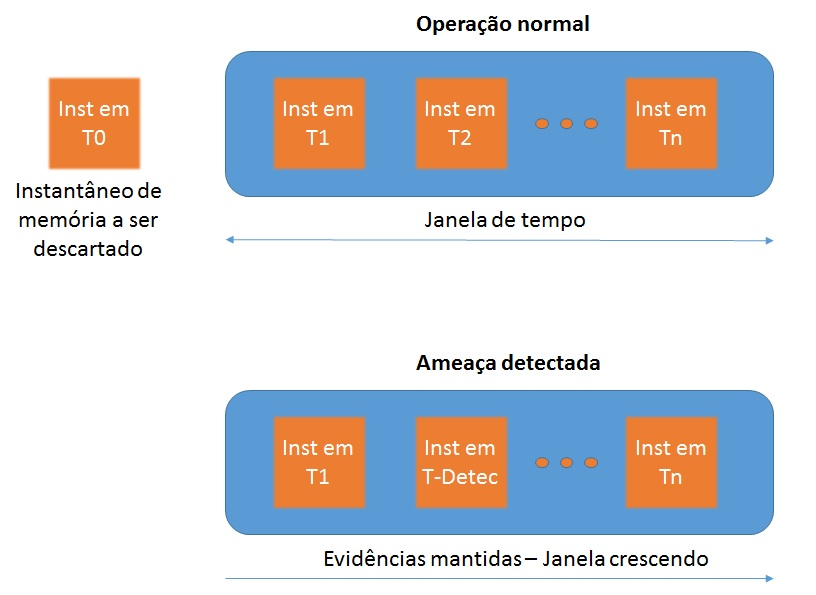
\includegraphics[scale=0.4]{janela.jpg}
\centering
\label{fig:janela}
\end{figure}

%\marcosT{Essa frase não faz sentido: não se ``assina'' nada com um ``hash''. Você pode ``calcular o hash'' ou ``assinar um dado'' (e.g., um dado juntamente com o hash de alguma coisa). Revise essa frase... - Hamilton: Feito}
Para persistir a relação evidência-origem e garantir a integridade da mesma, a presente proposta calcula o hash do par [evidência, identificador da imagem do contêiner] e armazena a tripla [hash, identificador da imagem do contêiner, evidência].
%
Para evitar eventuais problemas com o armazenamento desses dados em países com jurisdições diferentes daquelas que devem ser aplicadas na investigação em questão, as evidências coletadas são armazenadas em um local físico fora da nuvem, após serem transportadas por meio de um canal seguro (e.g., usando o protocolo \textit{Transport Layer Security} -- TLS \cite{DierksT2008}).
%

%

\subsection{Implementação}

%\marcosT{CLAREZA: quais ataques? Onde estão esses objetivos (diga a seção!!!)? Perceba que não tem qualquer seção com esse nome: você espera realmente que o leitor procure no seu texto onde eles estão...? - Hamilton: Feito}

Os métodos propostos foram implementados em uma plataforma de testes visando avaliar a eficácia de \fancyname em coletar as informações de memória dos contêineres de forma reprodutível, garantindo a cadeia de custódia sem violar jurisdições ou a privacidade de usuários.
%
A solução, ilustrada na Figura \ref{fig:Solucao}, consistiu na criação de 1 máquina virtual usando o Oracle Virtual Box 5.0 \cite{VirtualBox} em um notebook Intel i5 de 2.30Mhz e 4Gb de RAM com sistema operacional de 64 bits.
%
Essas máquinas virtuais possuem 2 Gb de memória RAM e emulam apenas 1 processador, e em cada uma delas foi instalado o Docker Engine 1.10 \cite{DockerInc} e a API Docker 1.21 \cite{DockerInc}, com os quais foram criados 3 contêiners executando o nginx 1.0 \cite{nginx} em diferentes portas. 
%
Usando uma aplicação Java que descobre qual o identificador de processo associado a cada contêiner, pode-se copiar conteúdo do \textit{descritor de alocação de memória não uniforme} (\textbf{/proc/pid/numa\_maps}) que contem a alocação das páginas de memória, os nós que estão associados a essas páginas, o que está alocado e suas respectivas políticas de acesso\cite{UnixManPages_numa_maps}. \marcosT{explique o que são esses dados! Hamilton - Feito}.
%
A cópia e gravação desse arquivo acontece da seguinte forma: a cada minuto, a aplicação (1) pausa o contêiner em questão, (2) copia a diretório \textbf{numa\_maps}, (3)  concatena os dados obtidos com o \textit{hash} de identificação da imagem do contêiner, (4) calcula o \textit{hash} do conjunto e (5) salva o resultado em um arquivo cujo nome é o identificador da imagem do contêiner e a extensão é \textbf{.mem}. 
%
Após a conclusão do processo de cópia, a mesma aplicação verifica se existem arquivos \textbf{.mem} em disco mais antigos do que um certo intervalo de tempo ``t'', descartando-os.
%

\marcosT{IMPORTANTE: discuta em alguns parágrafos os resultados. Até aqui, você só disse o que fez, mas não falou nada sobre o que isso traz de impactos positivos ou negativos. Por exemplo: quanto tempo demora a cópia (isso pode ser crítico para um processo que opera em tempo real, já que ele será pausado...)? Enfim, tire conclusões dos experimentos, porque senão os experimentos não têm qualquer utilidade para o leitor... Quanto mais completa a discussão (não só ``tempos'', mas também memória, quantidade de dados gerados por hora, uso de banda, etc.), melhor. Gráficos e tabelas com dados obtidos são muito bem vindos. - Hamilton: Feito}

\marcosT{IMPORTANTE: Discuta também a relação entre o que foi feito e os ataques de injeção mencionados na introdução. O seu texto inicialmente menciona tais ataques como parte do seu foco, mas nunca mais retoma a existência deles depois que você descreve a solução... Não precisa ser uma discussão longa, mas ao menos algumas considerações sobre o porquê de você conseguir analisar tais ataques usando a técnica proposta - Hamilton: Feito.}
%

%

\subsection{Experimento e Conclusões}

Para verificar se a presente proposta atinge os aos objetivos declarados montou-se o seguinte experimento.
%
A solução \fancyname foi configurada para realizar coletas de memória em intervalos de 1 minuto e apagar aquelas que tivessem mais de 5 minutos de existência. 
%
Permitiu-se que ela rodasse por 30 minutos. Durante este tempo foram coletadas métricas de uso de espaço em disco utilizado pelos instantâneos de memória salvos e o tempo de pausa no contêiner usado para a cópia das mesmas.
%
A cada coleta executou-se o comando \texttt{du -sh *.mem} do \textit{Unix} para retornar a lista dos instantâneos e o espaço em disco ocupado pelas coletas. 
%
Ao fim do experimento removeu-se os contêiners.


O espaço em disco ocupado pelos instantâneos de memória durante o experimento é mostrado na tabela \ref{tab:results-size} e plotado no gráfico \ref{fig:evolucao_coleta}. 
%
O gráfico mostra que o aumento do uso do espaço em disco é linear e o crescimento se interrompe quando é atingido o limite de tempo configurado para a janela pois as coletas com tempo de vida maior que tal limite são apagadas do disco. 
%
Podemos concluir que a solução mantem sob controle o espaço em disco ocupado pelas coletas.
%

\begin{table}[htb!]
\centering
\caption{Evolução do uso do espaço em disco}
\label{tab:results-size}
\begin{tabular}{c|c}
\hline
Tamanho total ocupado (KBytes) & Tempo (segundos) \\ \hline
240                            & 1                \\ \hline
480                            & 2                \\ \hline
720                            & 3                \\ \hline
960                            & 4                \\ \hline
1200                           & 5                \\ \hline
1200                           & 6                \\ \hline
1200                           & 7                \\ \hline
1200                           & 8                \\ \hline
1200                           & 9                \\ \hline
1200                           & 10                \\ \hline
1200                           & 11                \\ \hline
1200                           & 12                \\ \hline
1200                           & 13                \\ \hline
1200                           & 14                \\ \hline
1200                           & 15                \\ \hline
1200                           & 16                \\ \hline
1200                           & 17                \\ \hline
1200                           & 18                \\ \hline
1200                           & 19                \\ \hline
1200                           & 20                \\ \hline
1200                           & 21                \\ \hline
1200                           & 22                \\ \hline
1200                           & 23                \\ \hline
1200                           & 24                \\ \hline
1200                           & 25                \\ \hline
1200                           & 26                \\ \hline
1200                           & 27                \\ \hline
1200                           & 28                \\ \hline
1200                           & 29                \\ \hline
1200                           & 30                \\ \hline
\end{tabular}
\end{table}

\begin{figure}[htb!]
\caption{Evolução do uso do espaço em disco}
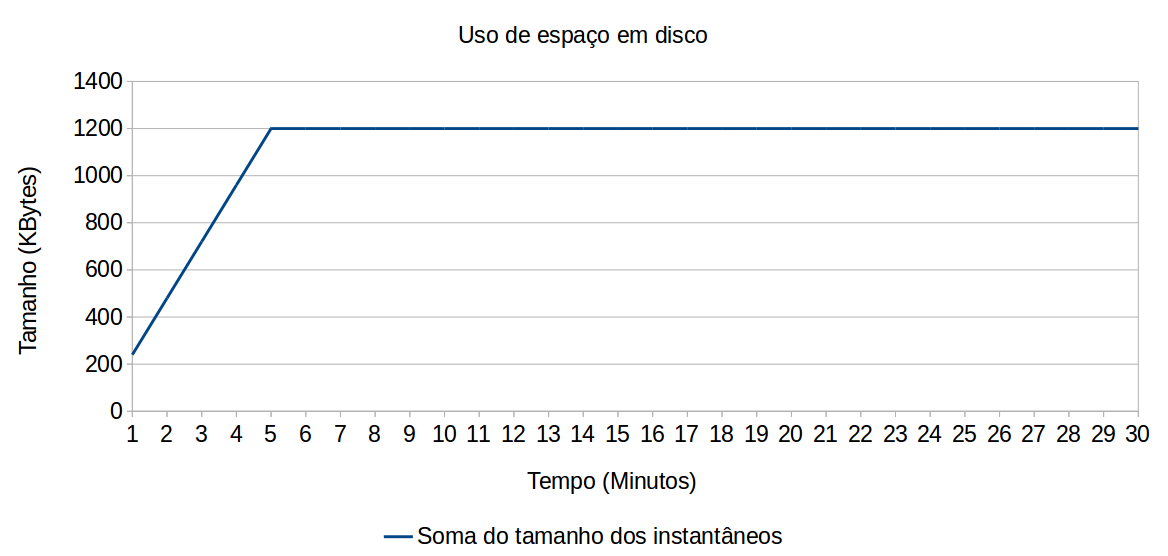
\includegraphics[scale=0.29]{evolucao_coleta.jpg}
\centering
\label{fig:evolucao_coleta}
\end{figure}


A figura \ref{fig:memoria_salva} é uma listagem de alguns dos instantâneos de memória salvos pela solução. Nela podemos ver que as coletas continuaram no disco da máquina mesmo após a remoção dos contêiners. Usando o identificador do contêiner e da imagem como nome do arquivo que armazena o instantâneo da memória conseguimos associar a evidência a sua origem.
%

\begin{figure}[htb!]
\caption{Lista de instantâneos de memória}
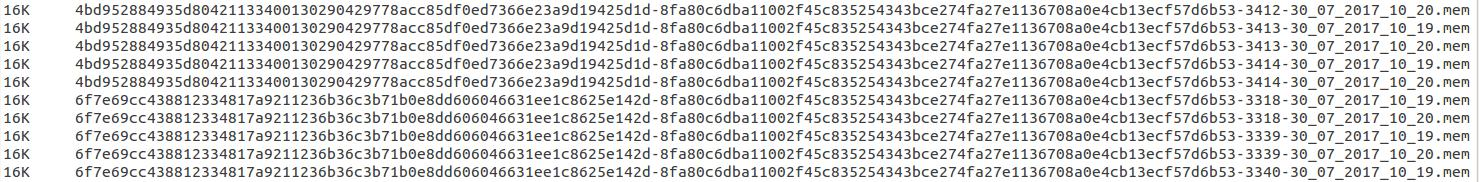
\includegraphics[scale=0.17]{memoria_salva.jpg}
\centering
\label{fig:memoria_salva}
\end{figure}


No evento da detecção de uma ameaça a presente proposta deixa de apagar as coletas mais antigas. Desta forma é capaz de descrever a história das alterações da memória do contêiner e com isso viabilizar a análise forense em busca das 4 vulnerabilidades de injeção de código citadas no início do artigo pois consegue descrever o estado do sistema antes e depois do incidente \cite{Case_Memory_Forensics:2014}.
%

Uma preocupação da presente proposta é o impacto que a pausa de um contêiner para coleta de dados pode causar na performance da aplicação executando no mesmo. A tabela \ref{tab:results-conteiner} mostra os tempos transcorridos para a cópia de memória durante o experimento. Os dados foram plotados no gráfico \ref{fig:memoria_copia}.
%
É possível notar que após a inicialização, o tempo para realizar a cópia da memória pela presente proposta no ambiente descrito na seção \textit{implementação} varia entre 20 e 40 milisegundos. 
%
Para avaliar o tempo de cópia deve-se levar em consideração o que está sendo executado no contêiner. 
%
Na implementação do presente experimento, cada contêiner está executando um motor de páginas web dinâmicas nginx 1.0 \cite{nginx}. Neste cenário o tempo gasto com a cópia é adequado. %encontrar referencia


\begin{table}[htb!]
\centering
\caption{Tempo de cópia da memória de um contêiner}
\label{tab:results-conteiner}
\begin{tabular}{c|c}
\hline
Tempo de cópia (Milisegundos) & Coleta           \\ \hline
149                           & 1                \\ \hline
59                            & 2                \\ \hline
23                            & 3                \\ \hline
32                            & 4                \\ \hline
35                            & 5                \\ \hline
21                            & 6                \\ \hline
17                            & 7                \\ \hline
38                            & 8                \\ \hline
16                            & 9                \\ \hline
33                            & 10               \\ \hline
17                            & 11               \\ \hline
36                            & 12               \\ \hline
18                            & 13               \\ \hline
25                            & 14               \\ \hline
31                            & 15               \\ \hline
14                            & 16               \\ \hline
33                            & 17               \\ \hline
19                            & 18               \\ \hline
13                            & 19               \\ \hline
20                            & 20               \\ \hline
18                            & 21               \\ \hline
24                            & 22               \\ \hline
8                             & 23               \\ \hline
9                             & 24               \\ \hline
19                            & 25               \\ \hline
7                             & 26               \\ \hline
8                             & 27               \\ \hline
11                            & 28               \\ \hline
35                            & 29               \\ \hline
13                            & 30               \\ \hline
\end{tabular}
\end{table}


\begin{figure}[htb!]
\caption{Lista de instantâneos de memória}
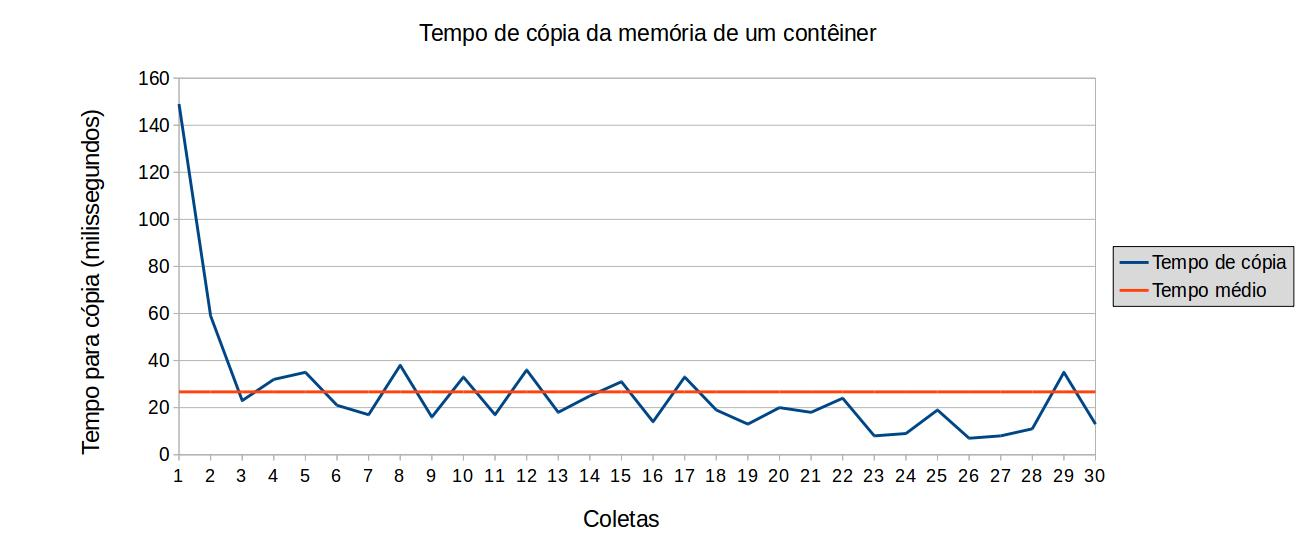
\includegraphics[scale=0.32]{memoria_copia.jpg}
\centering
\label{fig:memoria_copia}
\end{figure}

\subsection{Limitações}

Como a solução descrita tem como foco coletar informações de memória no espaço do usuário (\textit{user space}), ela não consegue acessar o espaço de kernel (\textit{kernel space}). 
%
Assim, \fancyname em princípio não provê suporte a técnicas de investigação de malware que se baseiam em informações do \textit{kernel space}, como, por exemplo, a comparação de informações do bloco do ambiente do processo (\textit{Process Environment Block -- PEB}), que ficam no \textit{user space}, com informações do descritor de endereços de memória virtual (\textit{Virtual Address Descriptor -- VAD}), que fica no \textit{kernel space}. 
%
Análise de ameaças que realizam manipulação direta dos objetos do kernel (D.K.O.M.-- \textit{Direct Kernel Object Manipulation}) também não se beneficiam com a solução aqui proposta. \marcosT{Não entendi a ``associação com o contêiner'' aqui. Você quer dizer que ``não se beneficiam com a solução aqui proposta'' ou outra coisa? Você não definiu o que seria a tal ``associação com o contêiner'' fora do contexto da sua solução, então ficou confuso - Hamilton: Feito}.

\begin{figure}[htb!]
\caption{Desenho completo da solução Dizang \marcosT{``Solução completa'' do que, cara pálida? Legendas devem ser auto-explicativas (i.e., se o leitor não ler sequer uma linha do seu texto e bater o olho em uma figura, ele deve conseguir entender alguma coisa daquela figura...) Com o nome ``Solução completa'', pode ser desde uma ``receita de bolo'' até a ``cura para o câncer''... - Hamilton: Feito}}
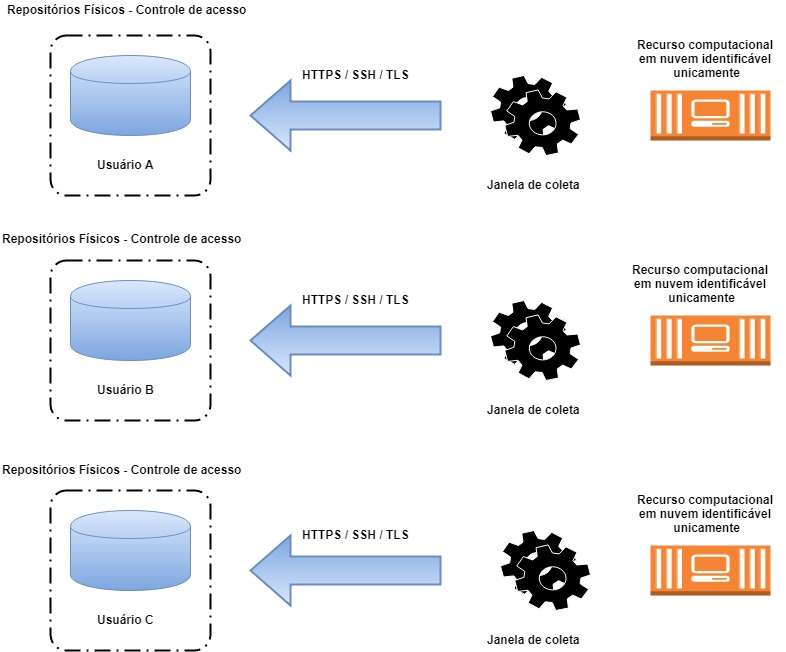
\includegraphics[scale=0.25]{solucao.jpg}
\label{fig:Solucao}
\end{figure}

% An example of a floating figure using the graphicx package.
% Note that \label must occur AFTER (or within) \caption.
% For figures, \caption should occur after the \includegraphics.
% Note that IEEEtran v1.7 and later has special internal code that
% is designed to preserve the operation of \label within \caption
% even when the captionsoff option is in effect. However, because
% of issues like this, it may be the safest practice to put all your
% \label just after \caption rather than within \caption{}.
%
% Reminder: the "draftcls" or "draftclsnofoot", not "draft", class
% option should be used if it is desired that the figures are to be
% displayed while in draft mode.
%
%\begin{figure}[!t]
%\centering
%\includegraphics[width=2.5in]{myfigure}
% where an .eps filename suffix will be assumed under latex, 
% and a .pdf suffix will be assumed for pdflatex; or what has been declared
% via \DeclareGraphicsExtensions.
%\caption{Simulation Results.}
%\label{fig_sim}
%\end{figure}

% Note that IEEE typically puts floats only at the top, even when this
% results in a large percentage of a column being occupied by floats.


% An example of a double column floating figure using two subfigures.
% (The subfig.sty package must be loaded for this to work.)
% The subfigure \label commands are set within each subfloat command,
% and the \label for the overall figure must come after \caption.
% \hfil is used as a separator to get equal spacing.
% Watch out that the combined width of all the subfigures on a 
% line do not exceed the text width or a line break will occur.
%
%\begin{figure*}[!t]
%\centering
%\subfloat[Case I]{\includegraphics[width=2.5in]{box}%
%\label{fig_first_case}}
%\hfil
%\subfloat[Case II]{\includegraphics[width=2.5in]{box}%
%\label{fig_second_case}}
%\caption{Simulation results.}
%\label{fig_sim}
%\end{figure*}
%
% Note that often IEEE papers with subfigures do not employ subfigure
% captions (using the optional argument to \subfloat[]), but instead will
% reference/describe all of them (a), (b), etc., within the main caption.


% An example of a floating table. Note that, for IEEE style tables, the 
% \caption command should come BEFORE the table. Table text will default to
% \footnotesize as IEEE normally uses this smaller font for tables.
% The \label must come after \caption as always.
%
%\begin{table}[!t]
%% increase table row spacing, adjust to taste
%\renewcommand{\arraystretch}{1.3}
% if using array.sty, it might be a good idea to tweak the value of
% \extrarowheight as needed to properly center the text within the cells
%\caption{An Example of a Table}
%\label{table_example}
%\centering
%% Some packages, such as MDW tools, offer better commands for making tables
%% than the plain LaTeX2e tabular which is used here.
%\begin{tabular}{|c||c|}
%\hline
%One & Two\\
%\hline
%Three & Four\\
%\hline
%\end{tabular}
%\end{table}


% Note that IEEE does not put floats in the very first column - or typically
% anywhere on the first page for that matter. Also, in-text middle ("here")
% positioning is not used. Most IEEE journals/conferences use top floats
% exclusively. Note that, LaTeX2e, unlike IEEE journals/conferences, places
% footnotes above bottom floats. This can be corrected via the \fnbelowfloat
% command of the stfloats package.

\section{Considerações Finais}
\label{sec:conclusion}

\marcosT{Uma boa conclusão retoma, logo na primeira frase, o problema que ela se propunha a resolver. Comece com uma ou mais frases nesse sentido, (nota: \textbf{sem} copiar+colar de outro ponto do texto). - Hamilton: Feito}
%
A proposta apresentada é capaz de relacionar o instantâneo de memória a sua origem utilizando o \textit{hash} calculado da imagem do contêiner como identificador da evidência armazenada, limita a quantidade de dados armazenados usando a implementação de janela de armazenamento e é capaz de descrever a memória antes e depois de um ataque viabilizando a análise de ataques de injeção de memória. 
%
Combinada com uma ferramenta adequada para análise das ameaças, essa característica de \fancyname pode ser uma ferramenta poderosa para análises forenses.
%
Cabe notar, entretanto, que muitas ferramentas de análise malware disponíveis no mercado necessitam que todo o conteúdo da memória da máquina esteja disponível para realização da análise com o FROST \cite{Dykstra_FROST:2013}, Volatility Framework \cite{VolatilityFoundation2014} e FATkit \cite{Fraser2006} (e.g., \marcosT{Dê exemplos com referências! - Hamilton: Feito}), o que inviabiliza seu uso diretamente sobre a memória de processos conforme coletado por \fancyname.
%
Portanto, como trabalho futuro, pretende-se desenvolver uma ferramenta mais flexível de análise, que, embora potencialmente utilize técnicas similares às atuais para detecção de ameaças, seja capaz de fazê-lo sem necessariamente ter acesso à memória completa da máquina.



\marcosR{As próximas frases, como escritas, são ``tiros no pé'': você fica falando das limitações que não são da sua proposta, mas sim do universo onde sua proposta se encaixa... Deixe a propaganda negativa para seus concorrentes fazerem, não para você... Refraseei para manter o mesmo conteúdo, mas de forma positiva em vez de negativa.}
%Apesar do sucesso em salvar a memória relacionadas ao contêiner e sua associação com a origem, não foi possível até o momento realizar uma análise das ameaças. 
%
%As ferramentas de análise de memória disponíveis no mercado necessitam que todo o conteúdo da memória da máquina esteja disponível para realização da análise. 
%
%Como é coletada apenas a memória relacionada aos processos, o ferramental não funciona. 
%
%É necessário o desenvolvimento de uma ferramenta que trabalhe sem a memória completa da máquina.

% trigger a \newpage just before the given reference
% number - used to balance the columns on the last page
% adjust value as needed - may need to be readjusted if
% the document is modified later
%\IEEEtriggeratref{8}
% The "triggered" command can be changed if desired:
%\IEEEtriggercmd{\enlargethispage{-5in}}

% references section

% can use a bibliography generated by BibTeX as a .bbl file
% BibTeX documentation can be easily obtained at:
% http://www.ctan.org/tex-archive/biblio/bibtex/contrib/doc/
% The IEEEtran BibTeX style support page is at:
% http://www.michaelshell.org/tex/ieeetran/bibtex/
\bibliographystyle{IEEEtran}
% argument is your BibTeX string definitions and bibliography database(s)
\bibliography{artigo-ieee}

% <OR> manually copy in the resultant .bbl file
% set second argument of \begin to the number of references
% (used to reserve space for the reference number labels box)

\end{document}


